\documentclass[tikz,border=10pt]{standalone}
\usepackage{tikz}
\usetikzlibrary{calc}
\begin{document}
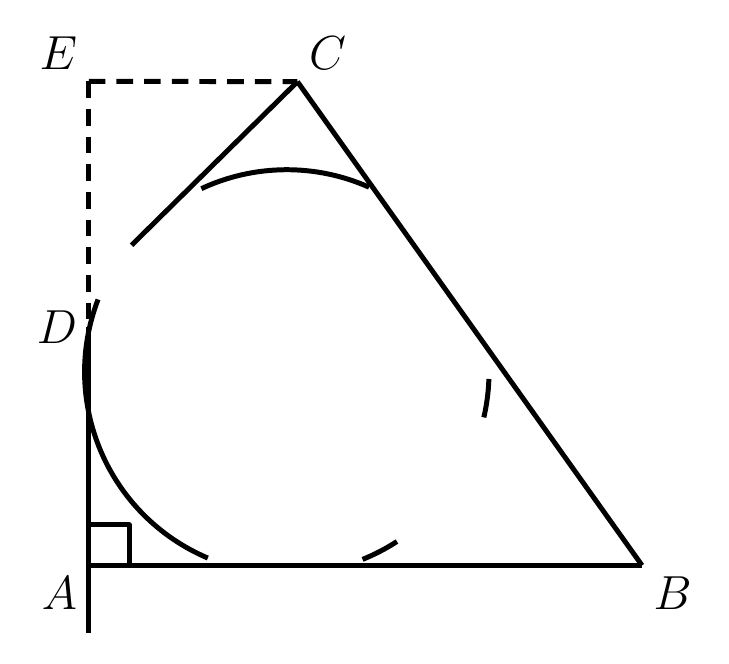
\begin{tikzpicture}[line width=1.8pt, line join=round]
  % Named coordinates (pixel -> cm, s = 0.022346, origin at A, y up)
  \coordinate (A) at (0,0);
  \coordinate (B) at (7.026,0);
  \coordinate (C) at (2.650,6.143);
  \coordinate (E) at (0,6.148);
  \coordinate (D) at (0,3.028);
  \coordinate (F) at (0.543,4.066);   % end of solid stroke from C
  \coordinate (Oc) at (2.515,2.457);  % arc centre
  \def\R{2.568}                        % arc radius

  % Solid segments
  \draw (A) -- (B);
  \draw (0,-0.86) -- (D);              % vertical A-D, overhang below A kept
  \draw (B) -- (C);
  \draw (C) -- (F);

  % Dashed segments
  \draw[dash pattern=on 6pt off 4pt] (E) -- (D);
  \draw[dash pattern=on 6pt off 4pt] (E) -- (C);

  % Right-angle mark at A
  \draw (0.514,0) -- (0.514,0.514) -- (0,0.514);

  % Visible arcs (math convention, y up)
  \draw ($(Oc)+(66:\R)$) arc[start angle=66, end angle=115, radius=\R];
  \draw ($(Oc)+(159:\R)$) arc[start angle=159, end angle=247, radius=\R];
  \draw ($(Oc)+(292:\R)$) arc[start angle=292, end angle=303, radius=\R];
  \draw ($(Oc)+(347:\R)$) arc[start angle=347, end angle=358, radius=\R];

  % Labels
  \node[font=\fontsize{17.5}{21}\selectfont, below left] at (A) {$A$};
  \node[font=\fontsize{17.5}{21}\selectfont, below right] at (B) {$B$};
  \node[font=\fontsize{17.5}{21}\selectfont, above right] at (C) {$C$};
  \node[font=\fontsize{17.5}{21}\selectfont, above left] at (E) {$E$};
  \node[font=\fontsize{17.5}{21}\selectfont, left] at (D) {$D$};
\end{tikzpicture}
\end{document}